% #############################################################################
% This is Appendix B
% !TEX root = ../main.tex
% #############################################################################
\chapter{Sefl-supervised learning models as feature extractor for children's \ac{ASR}}
\label{chapter:appendixB}

%\section{Introduction}
% Very short intro SSL
In light of the increasing availability of large amounts of unlabeled speech data, there has been a need to effectively extract general-purpose knowledge from such datasets. As a result, \ac{SSL} has experienced notable advances and garnered substantial attention in recent years, particularly in the context of leveraging large amounts of unlabeled speech data for low-resource annotated tasks. More formally, the \ac{SSL} paradigm refers to a training approach in which a model learns representations from unlabeled speech data without relying on explicit labels or annotations. This paradigm has yielded discernible enhancements in performance across various applications, such as speech recognition, speaker identification, and emotion recognition, to the point of achieving state-of-the-art results for some of these tasks \cite{baevski2020wav2vec}. Traditionally, \ac{SSL} models can be used in two manners: firstly, as a feature extraction method to replace human-designed features \cite{yang21c_interspeech,chang2021exploration}, and secondly, as a model initialisation accomplished by concatenating prediction layers and fine-tuning the entire model \cite{fan2022draft,jain2023wav2vec2,wang2021fine,li2021accent}.

% Children \ac{ASR} SSL
In recent years, an increasing amount of research has focused on using \ac{SSL} models for children \ac{ASR}. One notable avenue observed in the literature involves the fine-tuning of \ac{SSL} models using exclusively children's data \cite{jain2023adaptation} or through a combination of adult and children's data \cite{jain2023wav2vec2}. These efforts have yielded improved \ac{ASR} performances, showcasing the adaptability of \ac{SSL} models to the nuances inherent in the children's speech patterns. Conversely, an alternative strategy has emerged by using Adapters to help the \ac{SSL} model to specifically adapt to children's speech characteristics and subsequently followed by the full model, Adapters included, fine-tuning \cite{fan2022draft}. This initial training allows us to reduce the complexity associated with the conventional process of fine-tuning the entire model directly with children's speech.
%  Our motivation
The observed successes of \ac{SSL} as an initialization for fine-tuning in the context of children's \ac{ASR} underscore its efficacy as a new training paradigm. However, the exploration of \ac{SSL} models as front-end feature extractors, in comparison to conventional hand-crafted features, remains unexplored for children's \ac{ASR}, despite its use and success for adult speech \cite{yang21c_interspeech,chang2021exploration}. Motivated by these considerations, this annexe undertakes a comprehensive review of various \ac{SSL} models, evaluating their potential as novel feature extractors in the domain of children's \ac{ASR}.
\section{Self-supervised pre-trained models}

\begin{table}[htbp]
    \centering
    \begin{tabular}{ccccccc}
      \toprule
      Method & Architecture & \#Params & Stride & Input & Corpus & \\%Pretraining \\ 
      \midrule
      \multicolumn{6}{c}{\textbf{Hand-Crafted}} \\ \hline
      FBANK & - & 0 & 10ms & waveform & - & \\ \hline%- \\
      \multicolumn{6}{c}{\textbf{Generative}} \\ \hline
      Mockingjay \cite{mockingjay} & 12-Trans & 85.12M & 10ms & FBANK & LS 360 hr \\%& 360 hr time M-G \\
      Audio ALBERT \cite{chi2021audio} & 3-Trans & 7.15M  & 10ms & FBANK & LS 960 hr \\
      NPC  \cite{liu21l_interspeech} & 4-Conv, 4-Masked Conv & 19.38M & 10ms & FBANK & LS 360 hr \\%& 360 hr M-G + VQ \\
      APC \cite{chung19_interspeech} & 3-GRU & 4.11M & 10ms & FBANK & LS 360 hr \\%& 360 hr F-G \\
      TERA \cite{liu2021tera} & 3-Trans & 21.33M & 10ms & FBANK & LS 960 hr\\ \hline %& 960 hr time/freq M-G \\ 
      \multicolumn{6}{c}{\textbf{Discriminative}} \\ \hline
      Wav2Vec2 Base \cite{baevski2020wav2vec} & 7-Conv, 12-Trans & 95.04M & 20ms & waveform & LS 960 hr\\%& 960 hr M-C + VQ \\
      Wav2Vec2 Large \cite{baevski2020wav2vec} & 7-Conv, 24-Trans & 317.38M & 20ms & waveform & LL 60k hr\\%& 60k hr M-C + VQ \\
      Distill HuBERT \cite{chang2022distilhubert} & 7-Conv, 3-Trans & 23.49M & 20ms & waveform & LS 960 hr \\%& 960 hr M-P + VQ \\
      HuBERT Base \cite{hsu2021hubert} & 7-Conv, 12-Trans & 94.68M & 20ms & waveform & LS 960 hr \\%& 960 hr M-P + VQ \\
      HuBERT Large \cite{hsu2021hubert} & 7-Conv, 24-Trans & 316.61M & 20ms & waveform & LL 60k hr\\%& 60k hr M-P + VQ \\
      \bottomrule
    \end{tabular}
    \caption{Overview of different SSL architectures used as frozen feature extractors}
    \label{tab:SSL_models}

  \end{table}


Traditionally, \ac{SSL} models can be categorised into two distinct approaches: generative modelling and discriminative modelling. In this section, we will focus on summarising a selection of \ac{SSL} models used as front-end frozen feature extractors for our experiment. Further details of these \ac{SSL} models are presented in Table \ref{tab:SSL_models}, with a particular emphasis on their differences.

\subsection{Generative modeling}
% List a couple of models and explain their differences
Generative modelling has emerged as a prevalent approach for learning speech representations for \ac{SSL}. Generally, generative models are trained to generate speech frames based on their learned speech representations with or without the help of context. For instance, the \ac{APC} model \cite{chung19_interspeech} adopts a language model-like training paradigm, where a \ac{RNN} generates future frames predicted from the past frames. 
The Mockingjay model \cite{mockingjay} takes inspiration from \ac{BERT}-like pretraining techniques by masking input acoustic features along the time axis and subsequently regenerating the masked frames while the Audio ALBERT represent a smaller version of it \cite{chi2021audio}. Expanding upon this concept, the \ac{TERA} model \cite{liu2021tera} introduces an additional layer of complexity by masking bins in the frequency axis alongside the temporal axis. Finally, the \ac{NPC} model \cite{liu21l_interspeech} combines elements from both \ac{APC} and Mockingjay by substituting the \ac{RNN} in \ac{APC} with a \ac{CNN} layers and modifying the future frames generation process into a masked reconstruction.

\subsection{Discriminative modeling}
\begin{figure}[t]
    \centering
    \subfigure[Illustration of the Wav2vec2 architecture taken from \cite{baevski2020wav2vec}]{\label{fig:wav2vec2}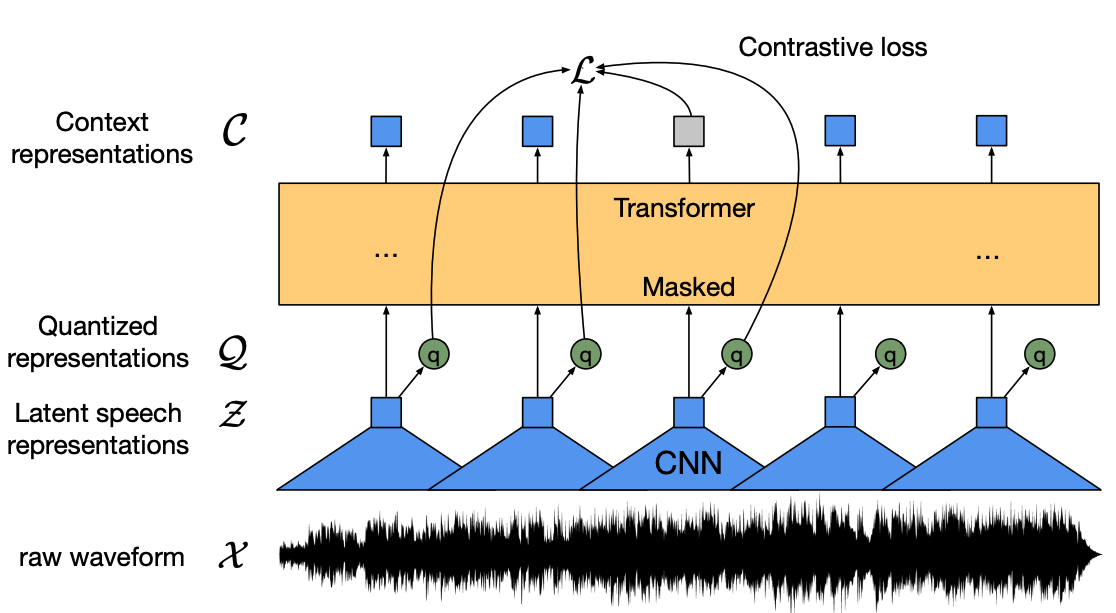
\includegraphics[width=0.48\textwidth]{imgs/wav2vec2.png}}
    \subfigure[Illustration of the HuBERT architecture taken from \cite{hsu2021hubert}]{\label{fig:Hubert}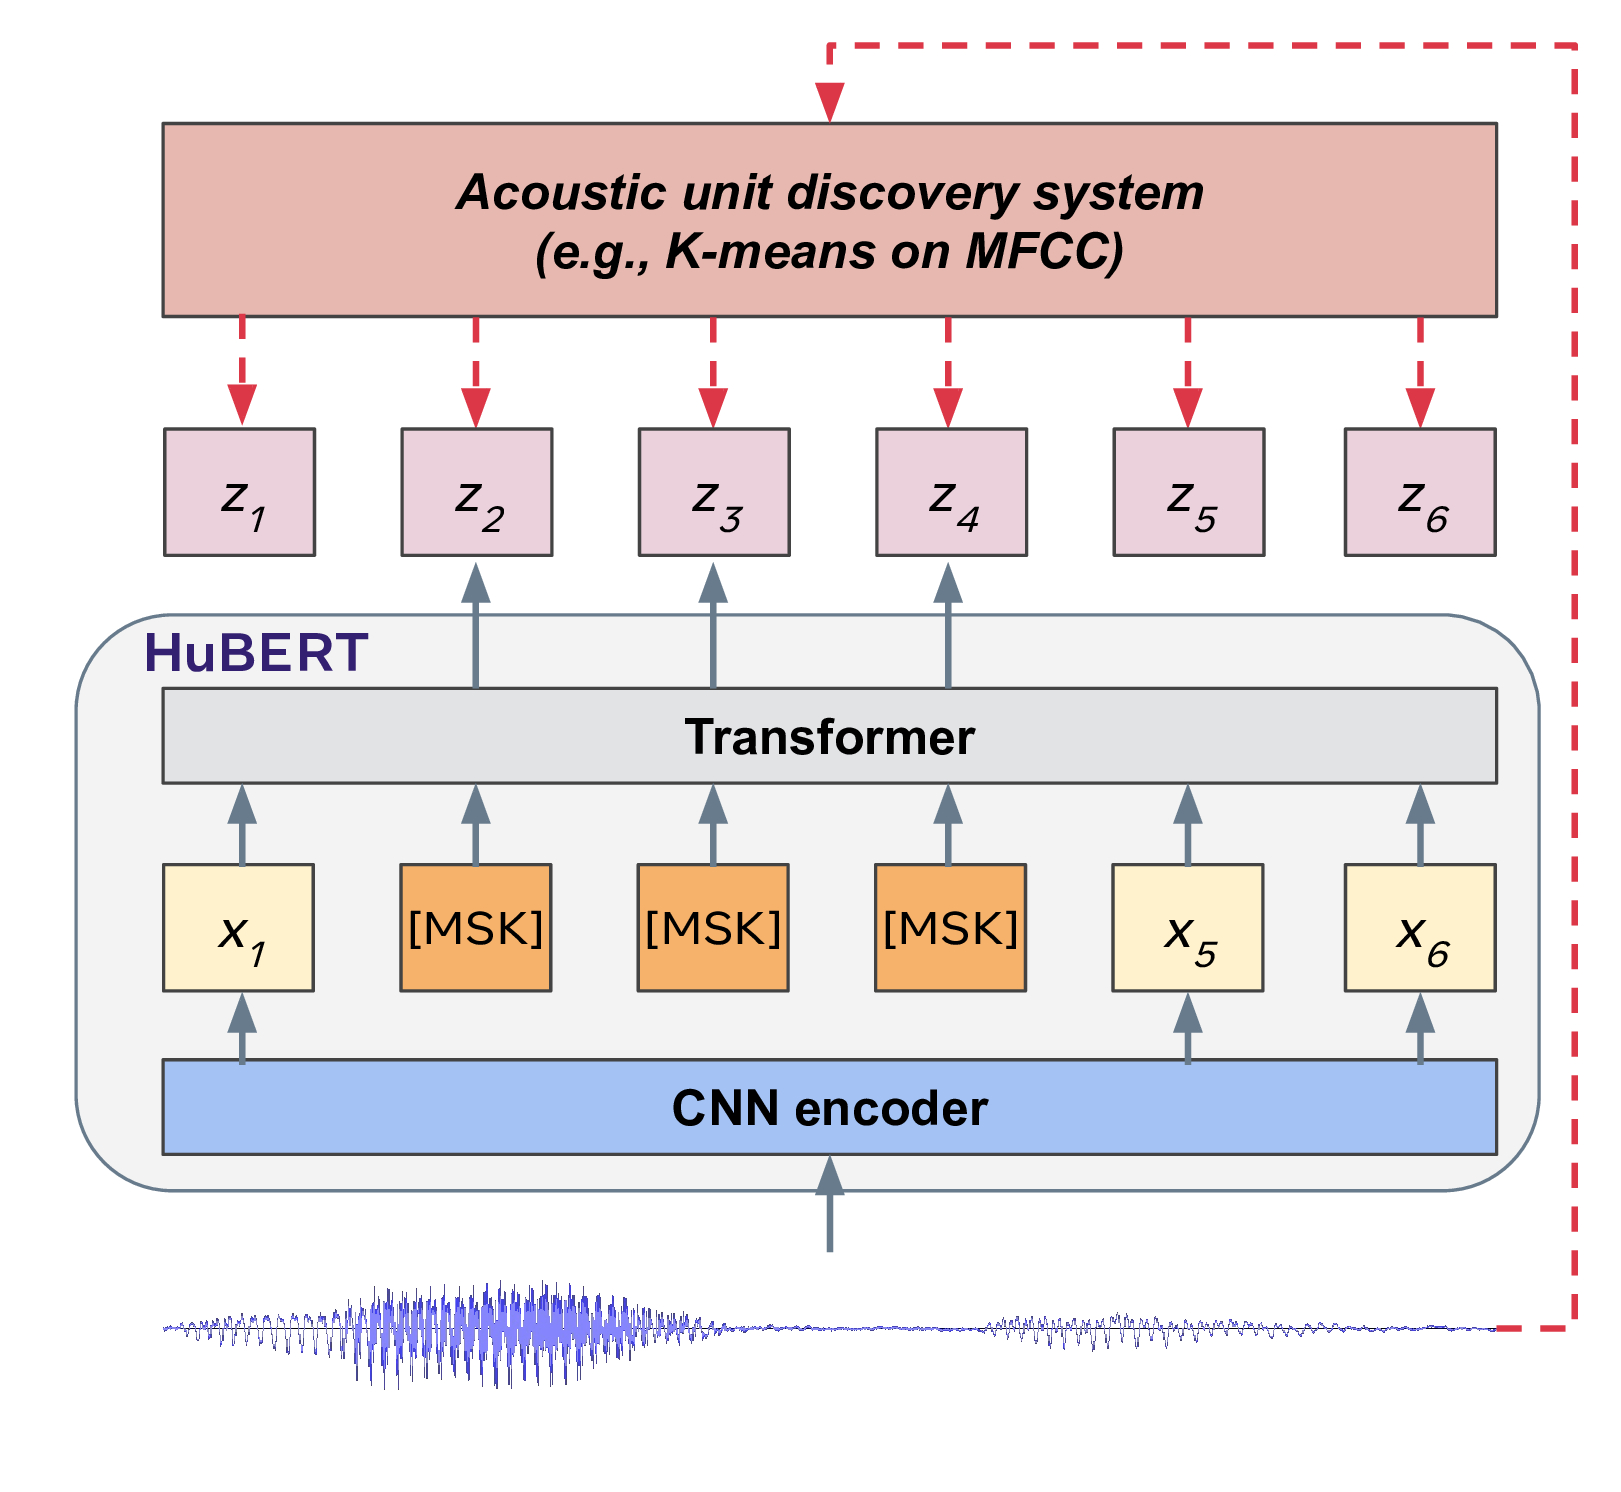
\includegraphics[width=0.48\textwidth]{imgs/Hubert.png}}
    \caption{Overview of the discriminative SSL Wav2vec2 and HuBERT models}
\end{figure}
% Explain Wav2Vec2 and Hubert    
The success of discriminative modelling has been notably pronounced with the introduction of the contrastive loss, which tries to discern between correlated positive samples and negative samples. The underlying intuition is that positive samples should exhibit closer representations in comparison to their negative counterparts. A prominent exemplar of the success of this approach is the Wav2Vec2 model \cite{baevski2020wav2vec}, which has demonstrated promising potential in learning speech representations. The Wav2Vec2 model achieves this by masking latent representations of the raw waveform and formulating a contrastive task over quantized speech representations. A more detailed representation of Wav2Vec2 architecture is displayed in figure \ref{fig:wav2vec2}. Later, moving away from the contrastive loss, the work of \cite{hsu2021hubert} proposed the HuBERT model. This model introduces a novel methodology by incorporating BERT's token prediction via offline clustering on representations. Specifically, the HuBERT model uses a \ac{BERT}-like training that consumes masked continuous speech features to predict pre-determined cluster assignments. The labels assigned to the masked locations during clustering serve as the predicted targets. Importantly, the predictive loss is selectively applied solely over the masked regions, compelling the model to learn robust high-level representations of unmasked inputs in order to accurately infer the targets of the masked ones. The HuBERT architecture is shown in figure \ref{fig:Hubert}. In our experiment, we also explore a distilled version of the HuBERT model, where the number of parameters is reduced \cite{chang2022distilhubert}.

\section{Experimental setup}
In our experimental setup, we used the Self-Supervised Speech Pre-training and Representation Learning (s3prl) toolkit\footnote{https://github.com/s3prl/s3prl} \cite{yang21c_interspeech}. The s3prl toolkit allows the modular use of pre-trained \ac{SSL} models, called upstream, to perform various downstream tasks, including \ac{ASR}. In order to evaluate the efficiency of different \ac{SSL} models as features extractors for children's \ac{ASR}, we froze the pre-trained \ac{SSL} models's weights to extract embedding representation of the children's speech signal as new acoustic features. All the different \ac{SSL} upstream models used in our experiments are listed along with detailed information regarding their architectures in table \ref{tab:SSL_models}. Notably, each of these models underwent self-supervised pre-training on either 360 or 960 hours of LibriSpeech \cite{librispeech} (denoted as LS 360hr and LS 960hr, respectively) or on an extensive 60 thousand hours of LibriLight data \cite{librilight} (referred to as LL 60k hr). 
The \ac{ASR} downstream task was conducted using a 2-layer Bidirectional \ac{LSTM} (BiLSTM) architecture with 1024 units, optimised with a \ac{CTC} loss. The training spanned 800 thousand iterations, with a learning rate set at $1.0\dot 10^{-4}$. Additionally, a dropout rate of $0.2$ was applied to the BiLSTM architecture to increase robustness. In these experiments, language models were not used. Additionally, limited by the large size of some \ac{SSL} model, we decided to use a subset of the Myst \cite{MyST} dataset, using 77 hours of speech for training, by removing the longest utterances in the train and validation sets. A detailed description of the filtered Myst data is provided in table \ref{tab:SSL_myst}.
\begin{table}[h!]

    
    \begin{center}
    \begin{tabular}{r|ccc}
    \hline
     & Training & Validation     & Test   \\ \hline
    \# of utterances & 23594   & 3959    & 4079  \\ 
    \# of speakers & 559  & 79    & 91  \\ 
    \# of hours & 77   & 12    & 13  \\ \hline
    \end{tabular}
    \caption{FilteredMy Science Tutor Children Speech Subset Corpus statistics used in the \ac{SSL} feature extraction experiment}
    \label{tab:SSL_myst}
    \end{center}
    \end{table}


\section{Results}

%For these models, the training process is separated into two stages. The first phase of training is self-supervised, which implies that no labels are used during training. The objective of this first phase is to present a large amount of unlabelled data to the system so that it learns a good speech representation. The second stage of learning is supervised fine-tuning, in which the model is taught to predict specific phonemes using the robust representation acquired in the previous stage with the help of a small amount of labelled data.
%In this category, two models stand out as state-of-the-art: Wav2Vec 2.0 \cite{baevski2020wav2vec} and HuBert \cite{hsu2021hubert}. As a preliminary experiment, to assess the usability of such frameworks for children \ac{ASR}, we trained a BiLSTM model using the output of a variety of frozen self-supervised systems. For this experiment, we used a subset of 50h of the Myst corpus \cite{MyST}, and the preliminary findings are displayed in the table \ref{tab:\ac{SSL}}
%\begin{table}[ht]
%\centering
%\begin{tabular}{lcc} 
%\hline
%\ac{SSL} upstream & UER $\downarrow$ & WER $\downarrow$ \\ 
%\hline
%Fbanks & 12.29\% & 35.14\% \\ 
%\hline
%Mockingjay & 12.49\% & 35.08\% \\
%APC & 11.88\% & 32.84\% \\
%TERA \cite{tera} & 11.31\% & 31.80\% \\
%Audio Albert \cite{chi2021audio} & 12.28\% & 34.69\% \\
%Wav2Vec2.0 Base & 7.37\% & 19.76\% \\
%Wav2Vec2.0 Large & 7.00\% & 18.76\% \\
%Distill HuBERT \cite{chang2022distilhubert} & 9.22\% & 25.75\% \\
%HuBERT Base & 7.40\% & 19.77\% \\
%HuBERT Large & \textbf{6.03\%} & \textbf{15.41\%} \\
%\hline
%\end{tabular}
%\caption{Results without language model of different Self-supervised models as feature extractors}
%\label{tab:\ac{SSL}}
%\end{table}

\begin{table}[ht]
  \centering
  \begin{tabular}{clcc}
  \hline
  Model type                      &  SSL upstream    & UER$\downarrow$ & WER $\downarrow$ \\ \hline
  Hand-crafted                    & Fbanks         & 12.29\%                                                           & 35.14            \\ \hline
  \multirow{4}{*}{Generative}     & Mockingjay     & 12.49\%                                                           & 35.08\%          \\
                                  & Audio Albert   & 12.28\%                                                           & 34.69\%          \\
                                  & NPC   & 11.99\%                                                           & 33.07\%          \\
                                  & APC            & 11.88\%                                                           & 32.84\%          \\
                                  & TERA           & 11.31\%                                                           & 31.80\%          \\ \hline
  \multirow{5}{*}{Discriminative} & Wav2Vec2 Base  & 7.37\%                                                            & 19.76\%          \\
                                  & Wav2Vec2 Large & 7.00\%                                                            & 18.76\%          \\
                                  & Distill HuBERT & 9.22\%                                                            & 25.75\%          \\
                                  & HuBERT Base    & 7.40\%                                                            & 19.77\%          \\
                                  & HuBERT Large   & \textbf{6.03\%}                                                   & \textbf{15.41\%} \\ \hline
  \end{tabular}
  \caption{Results without language model of different Self-supervised models as feature extractors}
\label{tab:SSL}
  \end{table}

Table \ref{tab:SSL} present the results of the comparison between various \ac{SSL} pre-trained models as feature extractors for children's \ac{ASR}. We provide \ac{UER} as well as \ac{WER}. In our experiment, the unit used for \ac{UER} were tokens. \ac{fbanks} are established as a baseline, yielding a \ac{UER} of 12.29\% and a \ac{WER} of 35.14\%. In terms of generative \ac{SSL} models, all configurations surpassed traditional \ac{fbanks} scores. Among the different generative \ac{SSL} models, APC  and \ac{TERA} exhibited the best performances in both \ac{UER}, 11.88\% and 11.31\% and \ac{WER} with 32.84\% and 31.80\% respectively. Turning to discriminative \ac{SSL} models, the Wav2Vec2 Base and Wav2Vec2 Large demonstrate substantial enhancements in performance compared to fbanks and generative models, achieving \ac{UER} values of 7.37\% and 7.00\%, and \ac{WER} of 19.76\% and 18.76\%, respectively. The distilled version of HuBERT outperforms \ac{fbanks} but falls behind the Wav2Vec2 models in terms of both \ac{UER} and \ac{WER} with 9.22\% \ac{UER} and 25.75\% \ac{WER}. Finally, HuBERT Base and HuBERT Large emerge as the best performing \ac{SSL} models, with the lowest \ac{UER} with respectively 7.40\% and 6.03\% and \ac{WER} of 19.77\% and 15.41\%. Notably, we observed that the best-performing models are the large discriminative pre-trained on a large amount of speech data.

The results suggest that large discriminative models, particularly HuBERT Large, demonstrate superior performance compared to other \ac{SSL} models and \ac{fbanks} as a feature extractor for children \ac{ASR}. Notably, even though no language model where used in this experiment, the results are of the same order as those reported in the different chapters of the thesis obtained with a Transformer and a Transformer language model. Showing the benefit of using frozen pre-trained \ac{SSL} models as feature extractors for children \ac{ASR}.

\section{Analysis of the extracted features}
\begin{figure}
  \begin{center}
  \centering
  \subfigure[]{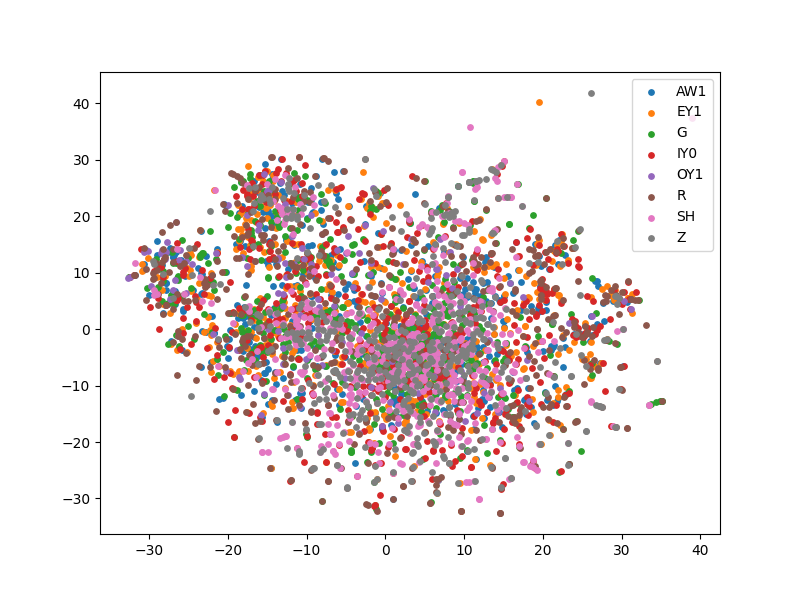
\includegraphics[width=0.49\textwidth]{imgs/fbank_umap_plot.png}} 
  \subfigure[]{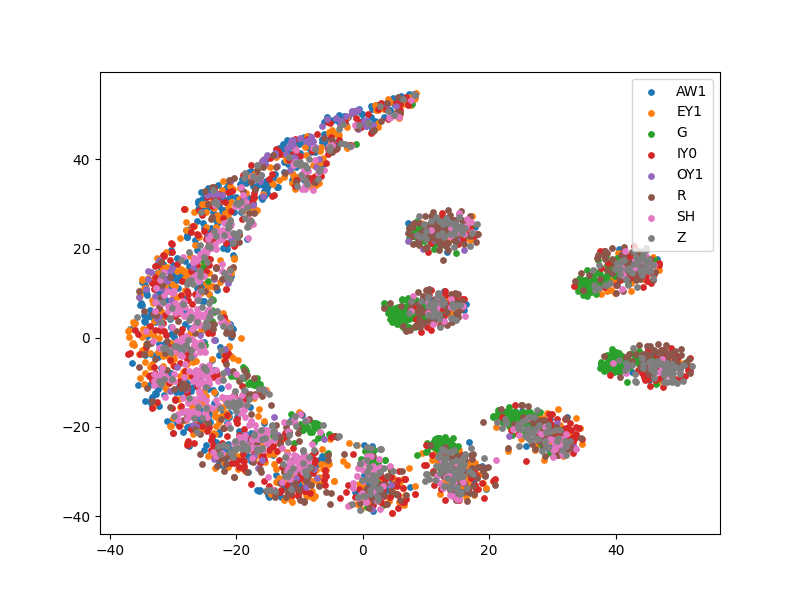
\includegraphics[width=0.49\textwidth]{imgs/tera_umap_plot.png}} 
  \subfigure[]{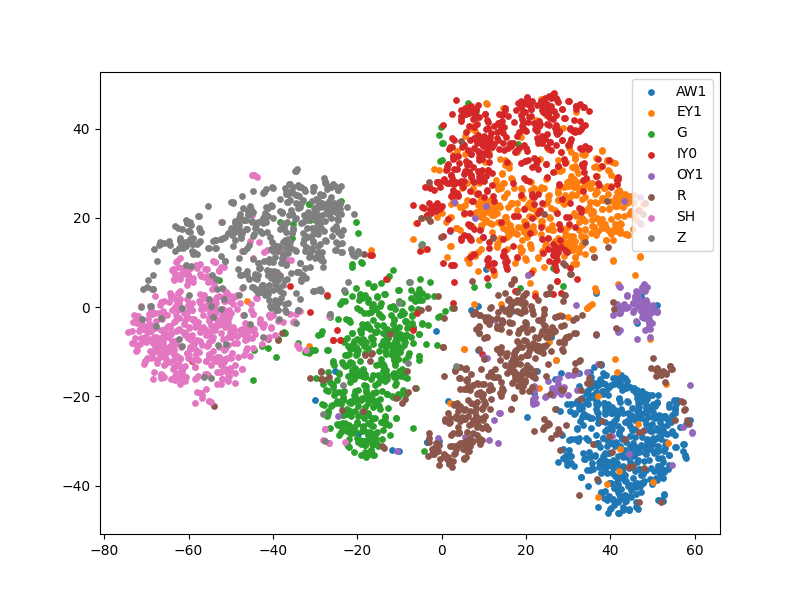
\includegraphics[width=0.49\textwidth]{imgs/wav2vec_umap_plot.png}}
  \subfigure[]{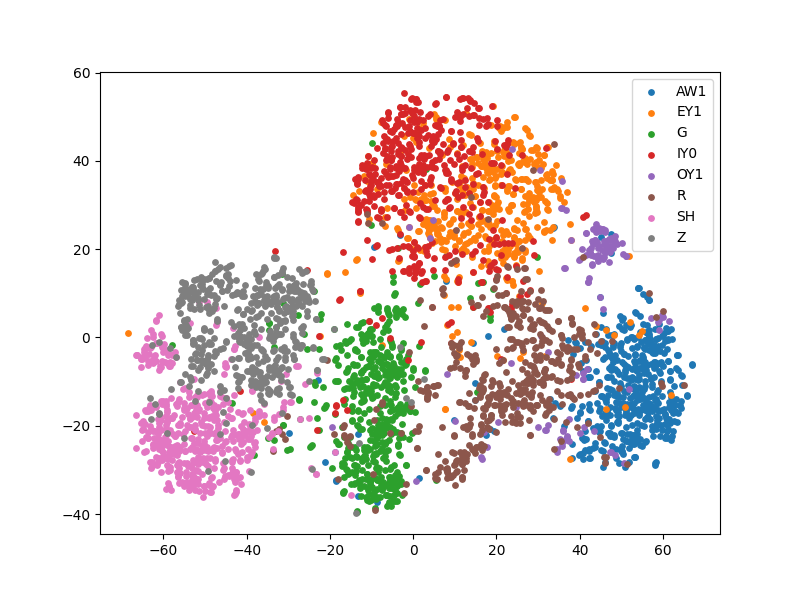
\includegraphics[width=0.49\textwidth]{imgs/hubert_umap_plot.png}}
  \caption{T-SNE plot of the different extracted features using the same speech data and their corresponding phoneme labels for: (a) Fbanks (b) TERA (c) Wav2Vec2 (d) HuBERT.}
  \label{fig:tsne_SSL}  
\end{center}
\end{figure}
% Explain experiment
In this section, we delve in more detail into the distinct features extracted from various models, aiming to better understand the notable performance differences observed between Wav2Vec2 and HuBERT, in contrast to \ac{TERA}, the best generative model in our experiment, and traditional filterbanks. To this end, we first aligned our children's speech data to obtain phoneme alignments using the Montreal Forced Aligner \cite{mcauliffe2017montreal}. %These phoneme alignments serve as the foundation for extracting different features corresponding to each phoneme.

% Explain the plot procedure
Therefore, the phoneme alignment is used to extract each phoneme present in an utterance. Then, we obtained variable-length \ac{SSL} feature sequences corresponding to the extracted features for the different frames where the phoneme has been aligned. In order to get a single vector for each phoneme uttered, we average these sequences. It is noteworthy that silence frames have been excluded. This operation is repeated for a subset of one thousand utterances of children's speech in order to gather different examples of the same phoneme from different speakers and different contexts. Subsequently, \ac{t-SNE} plots are generated for each of the studied models. 

% Plot interpretation
The \ac{t-SNE} plots are depicted in Figure \ref{fig:tsne_SSL}. We observe that traditional filterbanks features form a cloud point with no structure. This lack of structure suggests that the \ac{fbanks} features do not inherently exhibit phoneme-related information.
Moving to the \ac{t-SNE} plot of \ac{TERA} features, clusters are observable, but these clusters do not align with phonemes. This observation indicates that while \ac{TERA} features capture information from speech, they did not encode phoneme-specific information, as evidenced by the presence of mixed phonemes within the different clusters.
In contrast, both Wav2Vec2 and HuBERT exhibit highly similar plots, wherein distinct clusters corresponding to different phonemes are evident. This finding suggests that the features extracted from Wav2Vec2 and HuBERT inherently capture phonemic information, even though no explicit phoneme annotations were provided during training. The presence of these phoneme-related clusters indicates that the usage of these features facilitates the \ac{ASR} task by implicitly encoding phoneme information. We repeated this plotting procedure multiple times for different phoneme groups, and the same behaviour was observed. We note that these plots can help explain the different results observed in the previous section.


\section{Conclusions and future work}
% Conclusion 
In conclusion, the efficacy of \ac{SSL} across diverse tasks, motivated its utility as a pre-trained model for children's \ac{ASR}. However, these models are often large and can be difficult to fine-tune. Therefore, we proposed to use directly frozen pre-trained models as feature extractors in children's \ac{ASR}. Through a systematic exploration of feature types, including filter banks (fbanks), generative modelling, and discriminative modelling, we identified discriminative modelling as the most effective for children's \ac{ASR}. Specifically, the Wav2Vec2 and HuBERT models demonstrated a remarkable capability to implicitly encode phonemic information in their output representations, even in the absence of explicit phoneme information during training. Leveraging these explicit phonemes representation significantly contributes to enhancing the \ac{ASR} model's performance on children's speech, resulting in improved scores. This research contributes valuable insights towards a better use of pre-trained models for children's \ac{ASR} applications.

% Careful about the language used and future work
However, it is crucial to emphasise that the outcomes and findings of our experiments are highly dependent on the language used. Specifically, all the \ac{SSL} models were pre-trained using the English language, which aligns with the language of the children dataset used in this experiment. Consequently, the generalisability of our results may be limited when applied to different languages. Using a different language could potentially result in decreased performances, as the \ac{SSL} models may not be as adept at capturing the linguistic nuances and acoustic characteristics specific to that particular language \cite{phdthesis}. To address the language-dependent nature of our results, future work could explore the efficacy of employing multi-lingual \ac{SSL} models, such as XLS-R \cite{babu2021xlsr}. Moreover, a comparative analysis of the phonemic information explicitly encoded by discriminative models in children could be compared to the same extracted from adult speech. This exploration aims to discern whether an adult \ac{ASR} model, specifically trained using these phonetic features as input, could be directly applicable.  This avenue of research holds promise for advancing our understanding of model generalisation across different domains.

